\begin{document}
\maketitle

\begin{abstract}
\noindent Báo cáo nghiên cứu việc thay thế các reward term quy định dáng đi của policy
đi bộ cho robot hình người Unitree G1 trong \code{mjlab} bằng một reward học từ dữ liệu
mẫu theo hướng adversarial inverse reinforcement learning. Một discriminator được huấn
luyện để phân biệt transition của expert với transition của policy; đầu ra của nó được
dùng làm style reward, kết hợp với task reward bám vận tốc. Với reward kết hợp có tỉ
trọng style lớn, replay buffer cho discriminator, discriminator có điều kiện theo lệnh
và reference state initialization (RSI), policy đạt tracking error 0,20\,m/s (expert
0,16\,m/s), độ cao nhấc chân 5,7\,cm (expert 7,5\,cm) và 92\% tổng reward viết tay của
expert sau 2000 iteration, trong khi chưa từng được huấn luyện với các reward term này.
Thí nghiệm ablation cho thấy RSI là thành phần quyết định.
\end{abstract}

% ===========================================================================
\section{Bài toán}
% ===========================================================================
Điều khiển đi bộ được mô hình hóa là một MDP $(\mathcal{S}, \mathcal{A}, P, r, \rho_0,
\gamma)$. Tại mỗi bước $t$ ($\Delta t = 0{,}02$\,s), policy $\pi_\theta(a_t \mid o_t)$ nhận
quan sát $o_t$ (vận tốc thân, hướng trọng lực, góc và vận tốc 29 khớp, hành động trước
và lệnh vận tốc $c = (v_x^*, v_y^*, \omega_z^*)$) và xuất hành động $a_t \in \R^{29}$ là
độ lệch góc khớp so với tư thế mặc định. Policy được tối ưu bằng PPO~\cite{schulman2017ppo}
để cực đại hóa $J(\theta) = \E_{\pi_\theta}\big[\sum_t \gamma^t r_t\big]$ với
$\gamma = 0{,}99$.

Cấu hình gốc của \code{mjlab} dùng reward gồm 14 term viết tay: hai term bám vận tốc
\begin{equation}
  r^G_t = \Delta t\Big(2\,e^{-\|c_{xy} - v_{xy}\|^2 / 0{,}25}
  + 2\,e^{-(c_\omega - \omega_z)^2 / 0{,}5}\Big),
  \label{eq:task}
\end{equation}
với $v_{xy}$, $\omega_z$ là vận tốc dài và vận tốc xoay thực của thân, cùng 12 term quy
định dáng đi (thân thẳng, tư thế khớp, độ giật hành động, độ cao nhấc chân, trượt chân,
tự va chạm, \ldots). Ta gọi $r^G$ là \emph{task reward}.

\textbf{Mục tiêu.} Chỉ giữ $r^G$; thay 12 term dáng đi bằng \emph{style reward} $r^S$
học từ dữ liệu của một expert, sao cho policy đi theo lệnh với dáng đi giống expert và
hội tụ trong $\le 2000$ iteration.

% ===========================================================================
\section{Phương pháp}
% ===========================================================================
\subsection{Adversarial imitation learning (GAIL)}
Gọi $\rho_\pi$ là phân phối transition mà policy $\pi$ sinh ra. Imitation learning tìm
$\pi$ sao cho $\rho_\pi$ gần với phân phối của expert $\rho_E$. GAIL~\cite{ho2016gail}
đặt bài toán thành một trò chơi min--max giữa policy và một discriminator
$D_\psi : \mathcal{S} \times \mathcal{S} \to \R$ (đầu ra là logit $d$):
\begin{equation}
  \min_\pi \max_\psi \;
  \E_{(s,s') \sim \mathcal{D}_E}\big[\log \sigma(d)\big]
  + \E_{(s,s') \sim \pi}\big[\log(1 - \sigma(d))\big],
  \qquad d = D_\psi(s, s'),
  \label{eq:gail-game}
\end{equation}
với $\sigma$ là hàm sigmoid và $\mathcal{D}_E$ là tập transition của expert. Ở điểm tối ưu
của discriminator, giá trị hàm mục tiêu tương đương divergence Jensen--Shannon giữa
$\rho_\pi$ và $\rho_E$ (sai khác một hằng số), nên cực tiểu theo $\pi$ tương ứng với kéo
hai phân phối lại gần nhau.

\textbf{Discriminator} được huấn luyện như một bộ phân loại nhị phân:
\begin{equation}
  \mathcal{L}_D(\psi) = -\E_{\mathcal{D}_E}\big[\log \sigma(d)\big]
  - \E_{\mathcal{B}_\pi}\big[\log(1 - \sigma(d))\big]
  + \frac{w_\text{gp}}{2}\,\E_{\mathcal{D}_E}\big[\|\nabla_{(s,s')} d\|^2\big],
  \label{eq:disc}
\end{equation}
trong đó $\mathcal{B}_\pi$ là tập transition của policy và số hạng cuối là gradient
penalty~\cite{mescheder2018gp} ($w_\text{gp} = 10$), giữ $D$ trơn quanh dữ liệu expert.

\textbf{Style reward} là reward mà policy nhận được từ discriminator:
\begin{equation}
  r^S(s, s') = -\log\big(1 - \sigma(d)\big) = \log\big(1 + e^{d}\big).
  \label{eq:gail-reward}
\end{equation}
$r^S$ tăng đơn điệu theo xác suất $\sigma(d)$ mà discriminator gán cho việc transition
thuộc expert; cực đại hóa $r^S$ tương ứng với cực tiểu \eqref{eq:gail-game} theo $\pi$.
Policy và discriminator được cập nhật xen kẽ. Trong báo cáo này chỉ phần reward của GAIL
được dùng; policy được tối ưu bằng PPO thay cho TRPO của bài gốc.

\textbf{Discriminator trên transition.} GAIL gốc dùng cặp (trạng thái, hành động). Ở
đây discriminator nhận cặp trạng thái liên tiếp $(s_t, s_{t+1})$ (imitation from
observation), để không phụ thuộc vào không gian hành động của expert.

\textbf{Bão hòa.} Nếu discriminator phân biệt quá dễ ($d \ll 0$ trên dữ liệu policy)
thì $r^S \approx 0$ và gradient của nó theo trạng thái gần bằng 0: policy mất tín hiệu
style. Đây là chế độ thất bại chính của các cấu hình trước.

\subsection{Adversarial Motion Priors (AMP)}
AMP~\cite{peng2021amp} là một biến thể của GAIL cho điều khiển chuyển động. Khác biệt
chính nằm ở hàm mục tiêu của discriminator: thay entropy chéo bằng hồi quy bình
phương tối thiểu (least-squares GAN) về nhãn $+1$ cho expert và $-1$ cho policy,
\begin{equation}
  \mathcal{L}_D^\text{AMP} = \E_{\mathcal{D}_E}\big[(d - 1)^2\big]
  + \E_{\mathcal{B}_\pi}\big[(d + 1)^2\big] + \frac{w_\text{gp}}{2}\,
  \E_{\mathcal{D}_E}\big[\|\nabla d\|^2\big],
  \qquad
  r^S_\text{AMP} = \max\big(0,\; 1 - \tfrac14 (d - 1)^2\big).
  \label{eq:amp}
\end{equation}
Style reward của AMP bị chặn trong $[0, 1]$ và đạt cực đại khi $d = 1$ (giá trị gán cho
expert); reward của GAIL \eqref{eq:gail-reward} không bị chặn trên. AMP cũng đề xuất
replay buffer, RSI và đặc trưng vị trí bàn chân, bàn tay cho discriminator. Báo cáo so
sánh hai hàm mục tiêu này (\cref{sec:exp}).

\subsection{Kết hợp reward}
Reward đưa cho PPO là tổ hợp lồi của task reward và style reward:
\begin{equation}
  r_t = \lambda\, r^G_t + (1 - \lambda)\, w_S\,\Delta t\, r^S(s_t, s_{t+1}),
  \qquad \lambda = 0{,}3,\; w_S = 4,
  \label{eq:mix}
\end{equation}
theo Escontrela et al.~\cite{escontrela2022}. Hệ số $w_S \Delta t$ đưa $r^S$ về cùng
thang đo với $r^G$ (đã nhân $\Delta t$), để style chiếm khoảng 70\% tổng reward. Cặp
$(s_t, s_{t+1})$ nằm ở hai phía của một lần reset không phải là transition thật và bị
loại.

\subsection{Đặc trưng của discriminator}
Trạng thái đưa vào discriminator là $s = \Phi(\cdot) \in \R^{83}$, tính bằng cùng một
hàm cho expert và policy: vận tốc dài và vận tốc góc của thân trong hệ tọa độ thân
(6), hướng trọng lực trong hệ thân (3), độ cao thân (1), góc và vận tốc 29 khớp (58),
vị trí hai bàn chân và hai bàn tay so với thân trong hệ thân (12), và lệnh vận tốc $c$
(3). Việc đưa $c$ vào làm discriminator \emph{có điều kiện theo lệnh}: nó so sánh
chuyển động của policy với chuyển động của expert dưới cùng một lệnh, thay vì với phân
phối chuyển động gộp của mọi lệnh. Đầu vào được chuẩn hóa bằng trung bình và độ lệch
chuẩn của dữ liệu expert.

\subsection{Ổn định huấn luyện}
\begin{itemize}[leftmargin=*,itemsep=1pt]
  \item \textbf{Replay buffer.} $\mathcal{B}_\pi$ trong \eqref{eq:disc} được lấy mẫu từ
    một bộ đệm FIFO chứa $10^6$ transition gần nhất của policy, thay vì chỉ rollout của
    iteration hiện tại. Discriminator do đó không khớp quá mức với policy hiện tại, giảm
    bão hòa~\cite{peng2021amp}.
  \item \textbf{Không dùng entropy bonus.} Khi không còn term phạt độ giật, entropy bonus
    làm độ lệch chuẩn của hành động tăng liên tục; transition nhiễu dễ bị phân biệt và
    discriminator bão hòa. Độ lệch chuẩn ban đầu $\sigma_0 = 1$ được giữ để đủ khám phá.
\end{itemize}

\subsection{Reference State Initialization (RSI)}
Mỗi episode bắt đầu từ một trạng thái lấy từ phân phối ban đầu $\rho_0$ (ở đây: tư thế
đứng mặc định với nhiễu nhỏ). RSI~\cite{peng2021amp} thay $\rho_0$ bằng hỗn hợp với phân
phối trạng thái của dữ liệu mẫu:
\begin{equation}
  s_0 \sim (1 - p)\,\rho_0 + p\,\rho_E, \qquad p = 0{,}85 .
  \label{eq:rsi}
\end{equation}
Khi thu dữ liệu expert, ngoài đặc trưng $\Phi$ ta lưu trạng thái mô phỏng đầy đủ (độ
cao, hướng, vận tốc dài và góc của thân, góc và vận tốc khớp); khi một episode reset, với
xác suất $p$ robot được đặt vào một trạng thái như vậy. Policy do đó được huấn luyện ngay
từ đầu trên các pha của chu kỳ bước chân của expert, thay vì phải tự khám phá chúng từ
tư thế đứng --- điều khó xảy ra khi style reward đã thưởng cho việc đứng với tư thế giống
expert.

\subsection{Tóm tắt thuật toán}
\begin{figure}[H]
\centering
\begin{tikzpicture}[
  font=\small, node distance=6mm and 10mm,
  box/.style={draw,rounded corners,align=center,minimum height=10mm,
    text width=#1,fill=gray!6},
  box/.default=3.2cm,
  num/.style={circle,fill=black,text=white,inner sep=1pt,font=\scriptsize\bfseries},
  arr/.style={-{Stealth[length=2mm]},thick}]
  \node[box=3.4cm,fill=blue!6] (exp) {Expert $\pi_E$};
  \node[box=3.4cm,fill=blue!6,below=of exp] (data)
    {$\mathcal{D}_E$: $(s, s')$ và trạng thái mô phỏng};
  \draw[arr] (exp) -- node[right,font=\scriptsize]{rollout} (data);
  \node[num] at ($(exp.north west)+(0.1,0)$) {1};
  \node[box,right=18mm of exp,fill=green!6] (env) {Môi trường\\(4096 bản song song)};
  \node[box,right=20mm of env,fill=green!6] (pol) {Policy $\pi_\theta$};
  \node[box,below=of env,fill=orange!8] (disc) {Discriminator $D_\psi$\\ $\to r^S$};
  \node[box,below=of pol,fill=orange!8] (mix) {$r = \lambda r^G + (1-\lambda) w_S \Delta t\, r^S$};
  \node[box,below=of disc,fill=orange!8] (buf) {Replay buffer $\mathcal{B}_\pi$};
  \draw[arr] (pol) -- node[above,font=\scriptsize]{$a_t$} (env);
  \draw[arr] (env) -- node[left,font=\scriptsize,align=right]{$(s_t, s_{t+1})$} (disc);
  \draw[arr] (disc) -- node[above,font=\scriptsize]{$r^S_t$} (mix);
  \draw[arr] (env.south east) -- node[above right,font=\scriptsize,inner sep=1pt]{$r^G_t$} (mix.north west);
  \draw[arr] (mix.east) -- ++(0.4,0) |- node[right,pos=0.25,font=\scriptsize]{PPO} (pol.east);
  \draw[arr] (disc) -- (buf);
  \draw[arr] (data.east) -- ++(0.6,0) |- node[above,pos=0.75,font=\scriptsize]{mẫu expert} (disc.west);
  \draw[arr] (exp.east) -- node[above,font=\scriptsize]{RSI} (env.west);
  \draw[arr] (buf.east) -- ++(0.5,0) |- node[right,pos=0.25,font=\scriptsize]{mẫu policy} ($(disc.east)+(0,-0.2)$);
  \node[num] at ($(env.north west)+(0.1,0)$) {2};
  \node[num] at ($(disc.north west)+(0.1,0)$) {3};
  \node[num] at ($(mix.north west)+(0.1,0)$) {4};
  \node[num] at ($(pol.north west)+(0.1,0)$) {5};
  \node[num] at ($(buf.north west)+(0.1,0)$) {6};
\end{tikzpicture}
\caption{Luồng dữ liệu. Bước 1 thực hiện một lần; bước 2--6 lặp lại mỗi iteration.}
\label{fig:pipeline}
\end{figure}

\begin{enumerate}[leftmargin=*,itemsep=2pt]
  \item \textbf{Dữ liệu mẫu.} Chạy expert tất định trên 512 môi trường trong 10\,s với lệnh
    ngẫu nhiên; lưu $|\mathcal{D}_E| = 256\,000$ cặp $(s, s')$ và các trạng thái mô phỏng
    cho RSI. Expert là một policy PPO huấn luyện với đủ 14 reward term (3000 iteration).
  \item \textbf{Rollout.} 4096 môi trường $\times$ 24 bước; episode reset theo \eqref{eq:rsi};
    ghi $(s_t, s_{t+1})$ và $r^G_t$.
  \item \textbf{Style reward.} Tính $r^S$ theo \eqref{eq:gail-reward} (hoặc \eqref{eq:amp}).
  \item \textbf{Kết hợp} theo \eqref{eq:mix}.
  \item \textbf{Cập nhật policy} bằng PPO (GAE $\lambda = 0{,}95$, clip 0,2, 5 epoch $\times$
    4 mini-batch, learning rate $10^{-3}$ thích nghi theo KL).
  \item \textbf{Cập nhật discriminator.} Thêm transition của rollout vào $\mathcal{B}_\pi$;
    thực hiện 5 bước Adam (learning rate $10^{-4}$, batch 4096) trên \eqref{eq:disc} với mẫu
    từ $\mathcal{D}_E$ và $\mathcal{B}_\pi$.
\end{enumerate}
Policy và critic là MLP 512--256--128 (ELU); discriminator là MLP 1024--512 (ReLU).

% ===========================================================================
\section{Thí nghiệm}
\label{sec:exp}
% ===========================================================================
\textbf{Ablation.} Bốn cấu hình được huấn luyện song song trên một GPU, mỗi cấu hình
thêm một thành phần; các thiết lập còn lại giống hệt nhau (cùng expert, PPO, 4096 môi
trường, 2000 iteration, seed 42).

\begin{table}[H]
\centering
\small
\begin{tabular}{@{}lcccc@{}}
\toprule
 & Kết hợp \eqref{eq:mix} + replay buffer & Discriminator có điều kiện & RSI & Hàm mục tiêu $D$ \\
\midrule
v7a & \checkmark & & & GAIL \\
v7b & \checkmark & \checkmark & & GAIL \\
v7c & \checkmark & \checkmark & \checkmark & GAIL \\
v7d & \checkmark & \checkmark & \checkmark & AMP \\
\bottomrule
\end{tabular}
\end{table}
Mốc so sánh: expert và GAIL v4b --- cấu hình tốt nhất trước đó (reward cộng
$r^G + 2\Delta t\, r^S$, không replay buffer, không RSI, 1500 iteration, học từ một
expert cũ).

\textbf{Giao thức đánh giá.} Mọi policy được đánh giá trong cùng một lần chạy: 512 môi
trường $\times$ 1000 bước (20\,s), seed 123, lệnh ngẫu nhiên theo phân phối huấn luyện,
không đẩy robot, policy tất định. Các chỉ số:
\begin{itemize}[leftmargin=*,itemsep=1pt]
  \item \emph{Speed ratio} $v/v^* = \sum_t v_{xy}\!\cdot c_{xy} \,/\, \sum_t \|c_{xy}\|^2$
    (1: đúng lệnh; 0: đứng yên) và \emph{tracking error}
    $e = \overline{\|c_{xy} - v_{xy}\|}$ (m/s).
  \item \emph{Dáng bước} (khi $\|c_{xy}\| > 0{,}2$\,m/s): số lần chạm đất mỗi giây của mỗi
    bàn chân, và độ cao cực đại của bàn chân trong một bước.
  \item \emph{True reward} $\bar R$: tổng 14 reward term viết tay trên giây --- hàm reward
    mà các policy học (trừ expert) chưa từng được tối ưu.
\end{itemize}

% ===========================================================================
\section{Kết quả}
% ===========================================================================
\begin{table}[H]
\centering
\caption{Kết quả đánh giá tại iteration 2000.}
\label{tab:res}
\small
\begin{tabular}{@{}lcccccc@{}}
\toprule
 & $v/v^*$ $\uparrow$ & $e$ (m/s) $\downarrow$ & Chạm đất/s & Nhấc chân (cm) & $\bar R$ $\uparrow$ & $\bar R$ / expert \\
\midrule
Expert             & 0,84 & 0,16 & 2,0 & 7,5 & 5,03 & 100\% \\
GAIL v4b           & 0,81 & 0,18 & 6,6 & 1,4 & 3,18 & 63\% \\
\midrule
v7a                & 0,20 & 0,54 & 3,8 & 1,0 & 3,68 & 73\% \\
v7b                & 0,32 & 0,47 & 4,4 & 1,2 & 3,77 & 75\% \\
\textbf{v7c}       & \textbf{0,80} & \textbf{0,20} & \textbf{2,5} & \textbf{5,7} & \textbf{4,63} & \textbf{92\%} \\
v7d                & 0,17 & 0,57 & 2,8 & 3,1 & 3,63 & 72\% \\
\bottomrule
\end{tabular}
\end{table}

\begin{figure}[H]
\centering
\snap{Expert}{expert_step}
\snap{GAIL v4b}{gail_v4b}
\snap{v7c}{gail_v7c_it2000}
\caption{Lệnh tiến 0,5\,m/s, khung hình tại $t = 1, \dots, 5$\,s.}
\label{fig:snaps}
\end{figure}

\begin{figure}[H]
\centering
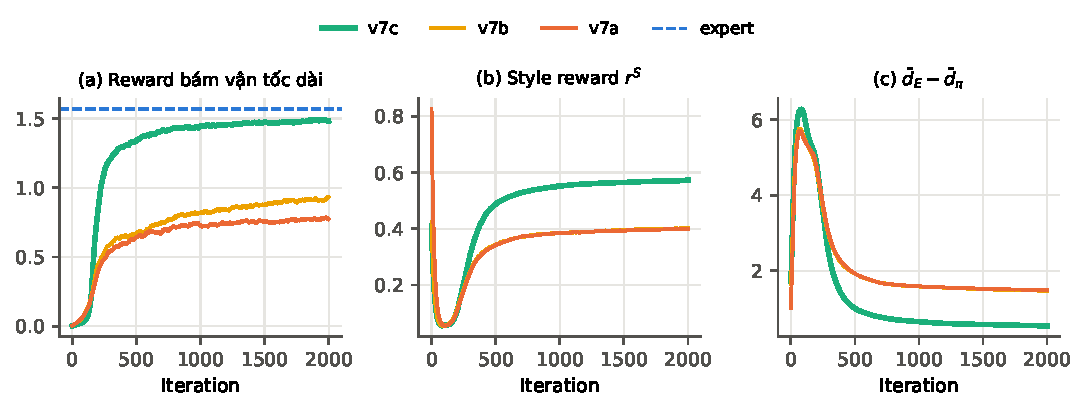
\includegraphics[width=\linewidth]{figures/simple_curves.pdf}
\caption{Diễn biến huấn luyện (làm mượt EMA). (a) Reward bám vận tốc dài trung bình
mỗi episode. (b) Style reward trung bình. (c) Hiệu $\bar d_E - \bar d_\pi$ giữa logit
trung bình của discriminator trên dữ liệu expert và trên dữ liệu policy.}
\label{fig:curves}
\end{figure}

\textbf{Cấu hình đầy đủ (v7c).} Policy đi theo lệnh gần mức expert ($v/v^* = 0{,}80$ so
với 0,84; $e = 0{,}20$ so với 0,16\,m/s) và đạt 92\% true reward của expert. So với GAIL
v4b, hiện tượng lê chân được khắc phục: số lần chạm đất giảm từ 6,6 xuống 2,5 lần/giây
(expert 2,0) và độ cao nhấc chân tăng từ 1,4 lên 5,7\,cm (expert 7,5). True reward tại
iteration 500 / 1000 / 1500 / 2000 lần lượt là 89\% / 91\% / 92\% / 92\% của expert: phần
lớn quá trình hội tụ diễn ra trong 500--1000 iteration đầu.

\textbf{Hội tụ của trò chơi đối kháng.} Với v7c, hiệu $\bar d_E - \bar d_\pi$ giảm dần về
gần 0 (\cref{fig:curves}c), tức discriminator ngày càng khó phân biệt transition của
policy với của expert, trong khi style reward giữ ở mức cao nhất trong các cấu hình
(\cref{fig:curves}b). Không cấu hình nào bị bão hòa.

\textbf{Ablation.}
\begin{itemize}[leftmargin=*,itemsep=2pt]
  \item \emph{RSI là thành phần quyết định.} Không có RSI (v7a, v7b), policy gần như
    đứng yên ($v/v^* \le 0{,}32$). Khi style reward chiếm phần lớn \eqref{eq:mix}, đứng
    với tư thế giống expert đã cho reward cao, và policy xuất phát từ tư thế đứng không
    khám phá được chu kỳ bước chân. RSI đưa policy vào các trạng thái của chu kỳ này
    ngay từ đầu.
  \item \emph{Discriminator có điều kiện} cải thiện nhẹ (v7b so với v7a).
  \item \emph{Hàm mục tiêu GAIL tốt hơn AMP} trên bài toán này (v7c so với v7d); nhất
    quán với các cấu hình trước.
\end{itemize}

\textbf{Khoảng cách còn lại so với expert:} độ cao nhấc chân (5,7 so với 7,5\,cm), tần số
bước (2,5 so với 2,0 lần/giây) và tốc độ (95\% của expert).

% ===========================================================================
\section{Kết luận}
% ===========================================================================
Một style reward học bằng adversarial imitation learning thay thế được 12 reward term
dáng đi viết tay cho bài toán bám vận tốc của G1: policy đạt 92\% true reward của
expert mà không được tối ưu trực tiếp trên nó, với dáng bước gần expert, trong 2000
iteration. Ba điều kiện cần là (i) style reward chiếm tỉ trọng lớn trong reward kết
hợp, (ii) discriminator được giữ khỏi bão hòa (replay buffer, không entropy bonus,
gradient penalty), và (iii) reference state initialization để policy tiếp cận chu kỳ
bước chân của expert.

\begin{thebibliography}{9}
\bibitem{ho2016gail} J.~Ho, S.~Ermon. Generative adversarial imitation learning.
  \emph{NeurIPS}, 2016.
\bibitem{peng2021amp} X.~B. Peng, Z.~Ma, P.~Abbeel, S.~Levine, A.~Kanazawa.
  AMP: Adversarial motion priors for stylized physics-based character control.
  \emph{ACM TOG (SIGGRAPH)}, 2021.
\bibitem{escontrela2022} A.~Escontrela, X.~B. Peng, W.~Yu, T.~Zhang, A.~Iscen,
  K.~Goldberg, P.~Abbeel. Adversarial motion priors make good substitutes for
  complex reward functions. \emph{IROS}, 2022.
\bibitem{mescheder2018gp} L.~Mescheder, A.~Geiger, S.~Nowozin. Which training
  methods for GANs do actually converge? \emph{ICML}, 2018.
\bibitem{schulman2017ppo} J.~Schulman, F.~Wolski, P.~Dhariwal, A.~Radford,
  O.~Klimov. Proximal policy optimization algorithms. \emph{arXiv:1707.06347}, 2017.
\end{thebibliography}

\end{document}
